% Machine translated from the Danish original, ../danish/dma-problems-2026-april.tex
\noindent\emph{This problem set has been machine translated from the Danish original.}
\medskip

\multiplechoicestart


\question{Arrays}
Let \(A[0:5] = \langle 3, 7, 1, 6, 2, 8 \rangle\) and \(B[1:4] = \langle 2, 5, 3, 1 \rangle\).
What is \(A[B[3] \cdot B[1] - 4]\)?
\oneanswer

\optionsstart
\answer The value is \(1\) \correct
\answer The value is \(2\)
\answer The value is \(3\)
\answer The value is \(6\)
\answer The value is \(7\)
\answer The value is \(8\)
\optionsend
\explanation{
We find \(B[3] = 3\) and \(B[1] = 2\).
The index becomes \(3 \cdot 2 - 4 = 2\).
Hence \(A[2] = 1\).
}

\question{Peaks in an array}
Which indices are peaks in the following array: \(A[1:5] = [5,7,7,3,3]\)?
Recall that an index \(i\) is a peak if \(A[i]\) is greater than or equal to all of its neighboring elements (each element has one or two neighbors).
\multipleanswers
\optionsstart
\answer Index \(1\)
\answer Index \(2\) \correct
\answer Index \(3\) \correct
\answer Index \(4\)
\answer Index \(5\) \correct
\optionsend
\explanation{
  Here \(A[2] = 7\) is greater than \(A[1] = 5\) and equal to \(A[3] = 7\),
  and \(A[3] = 7\) is equal to \(A[2] = 7\) and greater than \(A[4] = 3\).
  Therefore \(2\) and \(3\) are peaks.
  Since \(A[5]=3\) has only one neighbor, \(A[4]=3\), \(5\) is also a peak.
}


\question{Types of graphs}
Which of the following are terms from the course syllabus that describe a type of graph or a part of a graph?
\multipleanswers
\optionsstart
\answer node graph
\answer quadratic graph
\answer directed graph \correct
\answer tree \correct
\answer route
\answer cycle \correct
\optionsend
\explanation{
In the course we have encountered directed graphs, trees, and cycles, but the other terms are not standard terminology for types of graphs or parts of graphs.
}


\question{Data structures from the syllabus}
Which of the following are names of data structures from the course syllabus?
\multipleanswers
\optionsstart
\answer data net
\answer queue \correct
\answer collection
\answer hash table \correct
\answer total order
\optionsend
\explanation{
In the course we have studied queues and hash tables.
The other terms are not standard data structures.
}

\question{Sorting algorithms from the syllabus}
Which of the following are sorting algorithms from the course syllabus?
\multipleanswers
\optionsstart
\answer insertion sort \correct
\answer total sort
\answer counting sort \correct
\answer adaptive sort
\answer linear sort
\optionsend
\explanation{
Counting sort and insertion sort are classic sorting algorithms from the syllabus.
}

\question{Antisymmetric relation}
Let $X$ be a set and let $R \subseteq X \times X$ be a relation on $X$.
What does it mean for $R$ to be antisymmetric?
\oneanswer
\optionsstart
\answer $(a,b)\in R \Rightarrow a=b$
\answer $(a,b)\in R \Rightarrow (b,a)\notin R$
\answer $(a,b) \in R \land a\neq b \Rightarrow (b,a) \notin R$ \correct
\answer $(a,b) \in R \land (b,c) \in R \Rightarrow (c,a) \in R$
\optionsend
\explanation{
A relation $R$ is antisymmetric if $(a,b)\in R\land (b,a)\in R\Rightarrow a=b$, or equivalently $(a,b) \in R \land a\neq b \Rightarrow (b,a) \notin R$.
The other statements describe asymmetry or unnamed properties.
}
\pageshift

\question{Number of subsets}
How many subsets does a set with $10$ elements have?
\oneanswer
\optionsstart
\answer $\binom{10}{2}$
\itxanswer{binom(10,2)}
\answer $\binom{2}{10}$
\itxanswer{binom(2,10)}
\answer $10!$
\answer $2^{10}$ \correct
\answer $10$
\optionsend
\explanation{
The answer is $2^{10}$, since each element can either be in the subset or not.
}


\question{Number of orderings}
We have $20$ distinct playing cards in a hat.
We draw a card without putting it back, then draw another, and we continue like this until we have drawn $4$ cards.
How many different orderings of $4$ cards are possible?
\oneanswer
\optionsstart
\answer $20^4$
\answer $4^{20}$
\answer $20!/4!$
\answer $20!/16!$  \correct
\answer $\binom{20}{4}$
\itxanswer{binom(20,4)}
\answer $\binom{20}{16}$
\itxanswer{binom(20,16)}
\optionsend
\explanation{
There are $20$ choices for the first card, then $19$, then $18$, and finally $17$, which gives $20\cdot 19\cdot 18\cdot 17=20!/16!$ in total.
}

\question{Matrix computation}
Consider the following matrices:
\begin{align*}
    A =
\begin{bmatrix}
2 & 1\\
0 & 3\\
1 & 2
\end{bmatrix}
\quad \text{and} \quad
B =
\begin{bmatrix}
1 & 0\\
2 & 1\\
1 & 3
\end{bmatrix}.
\end{align*}

What is \(A^{T}B\)? (Here \(A^{T}\) is the transpose of \(A\).)
\oneanswer
\optionsstart

\answer \(\displaystyle \begin{bmatrix} 3 & 9\\ 3 & 9 \end{bmatrix}\)
\itxanswer{[[3,9],[3,9]]}

\answer \(\displaystyle \begin{bmatrix} 9 & 9\\ 3 & 3 \end{bmatrix}\)
\itxanswer{[[9,9],[3,3]]}

\answer \(\displaystyle \begin{bmatrix} 9 & 3\\ 9 & 3 \end{bmatrix}\)
\itxanswer{[[9,3],[9,3]]}

\answer \(\displaystyle \begin{bmatrix} 3 & 3\\ 9 & 9 \end{bmatrix}\) \correct
\itxanswer{[[3,3],[9,9]]}

\optionsend

\explanation{
We have
\begin{align*}
    A^{T} =
\begin{bmatrix}
2 & 0 & 1\\
1 & 3 & 2
\end{bmatrix}.
\end{align*}

Hence
\begin{align*}
A^{T}B &=
\begin{bmatrix}
2 & 0 & 1\\
1 & 3 & 2
\end{bmatrix}
\begin{bmatrix}
1 & 0\\
2 & 1\\
1 & 3
\end{bmatrix} \\
&=
\begin{bmatrix}
2\cdot1 + 0\cdot2 + 1\cdot1 & 2\cdot0 + 0\cdot1 + 1\cdot3\\
1\cdot1 + 3\cdot2 + 2\cdot1 & 1\cdot0 + 3\cdot1 + 2\cdot3
\end{bmatrix} \\
&=
\begin{bmatrix}
3 & 3\\
9 & 9
\end{bmatrix}.
\end{align*}
}

\question{Pseudocode}
Consider the following pseudocode
\begin{codebox}
\Procname{$\proc{Loop}(x)$}
\li $S \gets 0$
\li \For $i \gets 1$ \To $x$ \Do
\li \quad $S \gets S + 2i$
\li \quad $S \gets S - 1$
    \End
\li \Return S
\end{codebox}
What is returned when the code is called with input $x=3$?
\oneanswer
\optionsstart
\answer It returns 6
\answer It returns 9 \correct
\answer It returns 11
\answer It returns 12
\answer It returns 15
\optionsend
\explanation{
We start with $S=0$.
\begin{itemize}
    \item Iteration \(i = 1\): $S = 0 + 2\cdot1 = 2$, then $S = 2 - 1 = 1$
    \item Iteration \(i = 2\): $S = 1 + 4 = 5$, then $S = 5 - 1 = 4$
    \item Iteration \(i = 3\): $S = 4 + 6 = 10$, then $S = 10 - 1 = 9$
\end{itemize}
Hence $S = 9$ is returned.
}

\question{Markov's Inequality}
Let \(X\geq 0\) be a random variable for which we are told that $\mathbb E[X]=7/2$, and let $Y=4X$.
What upper bound can we give, using Markov's inequality, on the probability
\begin{align*}
  \Pr(Y \geq 20 )?
\end{align*}
\oneanswer

\optionsstart
\answer The upper bound is \(3/4\)
\answer The upper bound is \(2/3\)
\answer The upper bound is \(4/5\)
\answer The upper bound is \(7/10\) \correct
\optionsend

\explanation{
We have \(\mathbb{E}[Y] = 4 \cdot 7/2 = 14\).
We want to bound
\begin{align*}
  \Pr(Y \geq 20).
\end{align*}
To apply Markov's inequality we set
\begin{align*}
  a = \frac{20}{14} = \frac{10}{7},
\end{align*}
which gives
\begin{align*}
  \Pr(Y \geq 20) \leq \frac{1}{a} = \frac{7}{10}.
\end{align*}
}
\pageshift

\question{Representing a binary search tree in an array}
Let us represent a binary search tree in an array \(A[0:n-1]\) such that a node is stored
as four consecutive entries \(A[i:i+3]\), where \(A[i]\) is the key,
and \(A[i+1], A[i+2], A[i+3]\) are pointers to the parent, left child, and right child, respectively.
We store the root in the entries \(A[0:3]\).
The NIL pointer is written as a slash: \(/\).
Which of the arrays below represents the following binary search tree?

\begin{center}
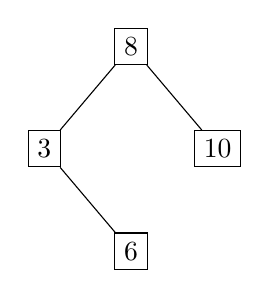
\begin{tikzpicture}[level distance=1.3cm, sibling distance=2.2cm]
  \node[draw,rectangle] {8}
    child {node[draw,rectangle] {3}
      child[missing]
      child {node[draw,rectangle] {6}}
    }
    child {node[draw,rectangle] {10}};
\end{tikzpicture}
\end{center}
\oneanswer

\optionsstart
\answer \(\langle 8, /, 4, 8, 3, 0, /, 12, 10, 0, /, /, 6, 4, /, / \rangle\) \correct
\answer \(\langle 8, /, 4, 8, 3, 0, 12, /, 10, 0, /, /, 6, 0, /, / \rangle\)
\answer \(\langle 8, /, 8, 4, 3, 0, 12, /, 10, 0, 12, /, 6, 4, /, / \rangle\)
\answer \(\langle 8, /, 8, 4, 3, 0, /, 12, 10, 0, 12, /, 6, 4, /, / \rangle\)
\answer \(\langle 8, /, 8, 4, 3, 0, /, 12, 10, 0, 12, /, 6, 0, /, / \rangle\)
\optionsend
\explanation{
  We use blocks of four entries per node, starting at indices \(0,4,8,12\).
  \begin{itemize}
    \item The root \(8\) is at \(A[0]\) with parent \(/\), left child \(4\) (the node \(3\)), and right child \(8\) (the node \(10\)).
    \item The node \(3\) is at \(A[4]\) with parent \(0\) (the root), no left child \((/)\), and right child \(12\) (the node \(6\)).
    \item The node \(10\) is at \(A[8]\) with parent \(0\) and no children.
    \item The node \(6\) is at \(A[12]\) with parent \(4\) and no children.
  \end{itemize}
  The array
  \(\langle 8, /, 4, 8, 3, 0, /, 12, 10, 0, /, /, 6, 4, /, / \rangle\)
  is the only one that corresponds to this tree.
}


\question{Pseudocode 2}
Consider the following pseudocode
\begin{codebox}
\Procname{$\proc{While-Loop}(x)$}
\li $y \gets 1$
\li $i \gets 0$
\li \While $i < x$ \Do
\li \quad $y \gets 2 \cdot y$
\li \quad $i \gets i + 1$
    \End
\li \Return $y$
\end{codebox}
Which function does the pseudocode compute when $x$ is a non-negative integer?
\oneanswer
\optionsstart
\answer $2x$
\answer $x^2$
\answer $2^x$ \correct
\answer $x^2+1$
\answer $x!$
\optionsend
\explanation{
The variable $y$ starts at $1$. In each iteration $y$ is multiplied by $2$, and the loop runs exactly $x$ times.
Hence the final value is
\[
y = 1 \cdot 2^x = 2^x.
\]
So the pseudocode computes the function $2^x$.
}

\question{Breadth-first search}
Consider the following directed graph $G$:

\begin{center}
\begin{tikzpicture}[>=Stealth, node distance=2.4cm]
    \tikzstyle{vertex}=[circle,draw,minimum size=18pt,inner sep=0pt]
    % Nodes
    \node[vertex] (A) {$A$};
    \node[vertex,right of=A] (B) {$B$};
    \node[vertex,right of=B] (C) {$C$};
    \node[vertex,below of=A,yshift=-0.8cm] (D) {$D$};
    \node[vertex,below of=B,yshift=-0.8cm] (E) {$E$};
    \node[vertex,below of=C,yshift=-0.8cm] (F) {$F$};

    % Edges
    \draw[->] (A) to (B);
    \draw[->] (A) to (D);
    \draw[->] (B) to (C);
    \draw[->] (B) to (E);
    \draw[->] (C) to (F);
    \draw[->] (E) to (D);
\end{tikzpicture}
\end{center}

From which source vertices will a breadth-first search (BFS) discover \emph{all} other vertices of the graph?
In other words, select the vertices $s\in\{A,B,\ldots,F\}$ such that the call $\proc{BFS}(G,s)$ colors all vertices black, where $\proc{BFS}(G,s)$ is the algorithm from CLRS Section 20.2.
\multipleanswers

\optionsstart
\answer \(A\) \correct
\answer \(B\)
\answer \(C\)
\answer \(D\)
\answer \(E\)
\answer \(F\)
\optionsend
\explanation{
  Starting at \(A\), we can reach \(B\) and \(D\). From \(B\) we can reach \(C\) and \(E\),
  and from \(C\) we can reach \(F\). Hence from \(A\) we can reach all of the vertices
  \(B, C, D, E, F\).

  None of the other vertices can reach \(A\), and several of them can reach only a few
  of the remaining vertices. Therefore \(A\) is the only vertex from which a BFS
  reaches all other vertices.
}


\question{Master Theorem}
Consider the following recurrence:
\begin{align*}
    T(1) & = 1 \\
    T(n) & = 2 \cdot T(\lceil n/2 \rceil) + 3 n^{3} \quad \text{for } n \geq 2.
\end{align*}
Using the Master Theorem, which of the following statements about \(T(n)\) is correct?
\oneanswer

\optionsstart
\answer \(T(n) = \Theta(n \log_{2} n)\)
\answer \(T(n) = \Theta(n^{2})\)
\answer \(T(n) = \Theta(n^{2} \log_{2} n)\)
\answer \(T(n) = \Theta(n^{3})\) \correct
\answer \(T(n) = \Theta(n^{3} \log_{2} n)\)
\optionsend
\explanation{
Here we have \(a = 2\), \(b = 2\), and \(f(n) = 3n^{3}\).
Hence
\begin{align*}
  n^{\log_{b} a} = n^{\log_{2} 2} = n.
\end{align*}
We see that
\begin{align*}
  f(n) = 3n^{3} = \Omega\bigl(n^{1+\varepsilon}\bigr)
\end{align*}
for example with \(\varepsilon = 2\).
Moreover, the regularity condition holds:
\begin{align*}
  a\,f(n/b)
  &= 2 \cdot 3 (n/2)^{3}
   = \frac{3}{4} n^{3}
   \le c \, n^{3}
\end{align*}
for a suitable \(c < 1\), e.g.\ \(\frac{3}{4}\).
Therefore we are in case 3 of the Master Theorem, and we get
\begin{align*}
  T(n) = \Theta\bigl(f(n)\bigr) = \Theta(n^{3}).
\end{align*}
}


\question{Insertion Sort}
Consider the following array \(A[1:6] = [5,2,4,6,1,3]\) and the pseudocode for \proc{Insertion-Sort} below.
How many times is the number 4 moved
(i.e.,~written somewhere in $A$) while sorting \(A\)?
\begin{codebox}
  \Procname{$\proc{Insertion-Sort}(A,n)$}
  \li \For $i \gets 2$ \To $n$ \Do
  \li $key \gets A[i]$
  \li $j \gets i-1$
  \li \While $j > 0$ and $A[j] > key$ \Do
  \li $A[j+1] \gets A[j]$
  \li $j \gets j-1$ \End
  \li $A[j+1] \gets key$
  \End
\end{codebox}
\oneanswer
\optionsstart
\answer It is moved \(0\) times
\answer It is moved \(1\) times
\answer It is moved \(2\) times
\answer It is moved \(3\) times \correct
\answer It is moved \(4\) times
\optionsend
\explanation{4 is moved three times. First when it is itself inserted
(line 7) into position 2, and then twice more when 1 and 3 are inserted in front of it.}


\question{Max-Heap}
You run \proc{Build-Max-Heap} on the array \(A[1:7] = \langle 5, 1, 9, 3, 7, 2, 6 \rangle\).
Which heap do you get as the result?
\oneanswer
\optionsstart
\answer \(\langle 9, 6, 7, 3, 2, 1, 5 \rangle\)
\answer \(\langle 9, 6, 7, 3, 1, 5, 2 \rangle\)
\answer \(\langle 9, 7, 6, 3, 1, 5, 2 \rangle\)
\answer \(\langle 9, 7, 6, 3, 1, 2, 5 \rangle\) \correct
\answer \(\langle 9, 7, 6, 3, 2, 1, 5 \rangle\)
\optionsend
\explanation{
Start: $A = \langle 5, 1, 9, 3, 7, 2, 6 \rangle$

After $\proc{Max-Heapify}(A,3)$:
$\langle 5, 1, 9, 3, 7, 2, 6 \rangle$

After $\proc{Max-Heapify}(A,2)$:
$\langle 5, 7, 9, 3, 1, 2, 6 \rangle$

After $\proc{Max-Heapify}(A,1)$:
First 5 and 9 are swapped:
$\langle 9, 7, 5, 3, 1, 2, 6 \rangle$

Then we continue from index 3, where 5 is swapped with 6:
$\langle 9, 7, 6, 3, 1, 2, 5 \rangle$
}
\pageshift

\question{Expected Value}
Let \(X_{1}, X_{2}, X_{3}\) be the outcomes of three independent rolls of a five-sided die with faces numbered from 1 to 5, each equally likely (we imagine that such a die exists).
What is the expected value of \(X_{1}\cdot X_{2}\cdot X_{3}\)?

\oneanswer
\optionsstart
\answer The expected value is 3
\answer The expected value is 5
\answer The expected value is 15
\answer The expected value is 25
\answer The expected value is 27 \correct
\optionsend
\explanation{The expected value of the product of independent random variables is the product of their expected values:
  \begin{align*}
    \mathbb{E}[X_{1}\cdot X_{2}\cdot X_{3}] =
    \mathbb{E}[X_{1}] \cdot \mathbb{E} [X_{2}] \cdot \mathbb{E} [X_{3}].
  \end{align*}
  The expected value of a single roll of a five-sided die is
  \begin{align*}
      \mathbb{E}[X_{i}] &=
      \frac{1+2+3+4+5}{5} = 3.
  \end{align*}
  So
  \begin{align*}
      \mathbb{E}[X_{1}\cdot X_{2}\cdot X_{3}] &=
      3 \cdot 3 \cdot 3 = 27.
  \end{align*}

}


\question{Heaps}
Consider this max-heap: $A[1:6]=\langle 99, 72, 70, 35, 7, 15\rangle$.
We can insert new values using \(\proc{Max-Heap-Insert}\).
If we insert the value \(76\),
at which index does it end up?
\oneanswer
\optionsstart
\answer Index 1
\answer Index 2
\answer Index 3 \correct
\answer Index 4
\answer Index 5
\answer Index 6
\answer Index 7
\optionsend
\explanation{We first insert 76 at index 7.
  Then we compare it with its parent at position 3 (70).
  Since \(76 > 70\), we swap them.
  Next we compare 76 with its new parent at index 1 (99).
  Since \(76 < 99\), the algorithm terminates, with 76 at index 3.}


\question{Disjoint sets}
We consider a partition of the numbers $\{0,1,\ldots,6\}$ into disjoint subsets.
The sets are represented as a forest given by the array representation
\[
P[0:6] = \langle 2, 3, 2, 3, 2, 5, 0 \rangle,
\]
where \(P[i]\) denotes the parent of element \(i\).

What are the sets?
\oneanswer

\optionsstart
\answer \(\{0,1,2\},\{3,4,5\},\{6\}\)
\answer \(\{0,1,2\},\{3\},\{4,5\},\{6\}\)
\answer \(\{0,2,4,6\},\{1,3\},\{5\}\) \correct
\answer \(\{0,1,2,4,6\},\{3\},\{5\}\)
\optionsend

\explanation{
We see that 2 is the parent of 0 and 4, and that 0 is the parent of 6, so one of the sets is \(\{0,2,4,6\}\).
The parent of 1 is 3, and 5 is its own parent, so the other sets are \(\{1,3\}\) and \(\{5\}\).
}


\question{Relations}
Consider the following relation \(R\) on the set of integers \(\mathbb{Z}\):
\begin{align*}
    m R n \iff | m - n | \leq 5
\end{align*}
Which properties does the relation $R$ have?
\multipleanswers

\optionsstart
\answer antisymmetric
\answer symmetric \correct
\answer reflexive \correct
\answer transitive
\optionsend
\explanation{The relation is not antisymmetric, since for example $0\, R\, 5$ and $5\, R\, 0$, but $0\neq 5$.
The relation is reflexive, since \(|m - m| = 0 \leq 5\) for all \(m \in \mathbb{Z}\).
The relation is symmetric, since \(|m - n| = |n - m|\) for all \(m,n \in \mathbb{Z}\).
The relation is not transitive, since for example $0\, R\, 5$ and $5\, R\, 10$, but \(| 0 - 10 | > 5\).}

\question{Combinatorics}
10 students are to be divided into groups of sizes 5, 3, and 2,
so that each student is in exactly one group.
In how many different ways can this be done?
\oneanswer

\optionsstart
\answer \(10^5\)
\answer \(10!\)
\answer \(\binom{10}{5} \cdot \binom{5}{3}\) \correct
\itxanswer{binom(10,5)*binom(5,3)}
\answer \(10^{5} \cdot 5^{3}\)
\answer \(5! \cdot 3! \cdot 2!\)
\answer \(\binom{10}{5} \cdot \binom{10}{3} \cdot \binom{10}{2}\)
\itxanswer{binom(10,5)*binom(10,3)*binom(10,2)}
\optionsend
\explanation{
  First we choose which 5 students are in the group of 5:
  \(\binom{10}{5}\) possibilities.
  From the remaining 5 we choose 3 for the group of three:
  \(\binom{5}{3}\) possibilities.
  The last 2 students automatically form the group of two, so there is only 1 possibility left.
  In total this gives
  \(\binom{10}{5} \cdot \binom{5}{3}\) ways.
}
\pageshift

\question{Dijkstra's algorithm}
Consider the following weighted, directed graph:

\begin{center}
\begin{tikzpicture}[>=Stealth, node distance=2.4cm]
  \tikzstyle{vertex}=[circle,draw,minimum size=18pt,inner sep=0pt]

  \node[vertex] (A) at (0,0) {A};
  \node[vertex] (B) at (2,1) {B};
  \node[vertex] (C) at (2,-1) {C};
  \node[vertex] (D) at (4,1) {D};
  \node[vertex] (E) at (4,-1) {E};

  \draw[->] (A) -- node[above] {1} (B);
  \draw[->] (A) -- node[below] {4} (C);
  \draw[->] (B) -- node[above] {5} (D);
  \draw[->] (B) -- node[right] {2} (C);
  \draw[->] (C) -- node[below] {1} (E);
  \draw[->] (D) -- node[right] {1} (E);
\end{tikzpicture}
\end{center}

Suppose Dijkstra's algorithm is used to find shortest paths from the vertex \(A\)
to all vertices of the graph.
Give the order in which the vertices are extracted from
the priority queue in Dijkstra's algorithm.
\oneanswer

\optionsstart
\answer \(A B C D E\)
\answer \(A B C E D\) \correct
\answer \(A B D C E\)
\answer  $A C B D E$
\answer \(A C B E D\)
\answer  $A C E B D$
\optionsend

\explanation{
\begin{itemize}
    \item Start: \(d(A)=0\), all others \(\infty\)
    \item From \(A\): \(d(B)=1\), \(d(C)=4\), so we choose \(B\)
    \item From \(B\): \(d(C)=1+2=3\), \(d(D)=1+5=6\)
    \item Next: \(C\) (distance \(3\))
    \item From \(C\): \(d(E)=3+1=4\)
    \item Next: \(E\) (distance \(4\))
    \item Last: \(D\) (distance \(6\))
\end{itemize}

The order is \(A,B,C,E,D\).
}


\question{Strongly connected components}
Consider the following directed graph:

\begin{center}
\begin{tikzpicture}[>=Stealth, node distance=2.2cm]
  \tikzstyle{vertex}=[circle,draw,minimum size=18pt,inner sep=0pt]

  \node[vertex] (A) at (0,0) {A};
  \node[vertex] (B) at (2,1) {B};
  \node[vertex] (C) at (2,-1) {C};
  \node[vertex] (D) at (4,1) {D};
  \node[vertex] (E) at (4,-1) {E};
  \node[vertex] (F) at (6,1) {F};
  \node[vertex] (G) at (6,-1) {G};
  \node[vertex] (H) at (8,0) {H};

  % SCC 1: A, B, C
  \draw[->] (A) -- (B);
  \draw[->] (B) -- (C);
  \draw[->] (C) -- (A);

  % SCC 2: D, E, G, H (cycle)
  \draw[->] (D) -- (E);
  \draw[->] (E) -- (H);
  \draw[->] (H) -- (D);
  \draw[->] (H) -- (D);
  \draw[->] (E) -- (G);

  % extra edges inside SCC 2 (to make it less obvious)
  \draw[->, bend left=15] (E) to (D);
  \draw[->, bend left=15] (G) to (E);

  % connections between SCCs
  \draw[->] (C) -- (D);
  \draw[->] (H) -- (F);
  \draw[->] (D) -- (F);
\end{tikzpicture}
\end{center}

Which of the following partitions corresponds to the strongly connected components of the graph?
\oneanswer

\optionsstart
\answer \(\{A,B,C,D,E,F,G,H\}\)
\answer \(\{A,B,C\}, \{D,E,G,H\}, \{F\}\) \correct
\answer \(\{A,B,C\}, \{D,E,F,G,H\}\)
\answer \(\{A,B\}, \{C,D\}, \{E,G\}, \{F,H\}\)
\answer \(\{A,B\}, \{C,D,F,H\}, \{E,G\}\)
\optionsend

\explanation{
A strongly connected component is a maximal set of vertices such that there are paths in both directions between every pair of them.

\begin{itemize}
    \item \(A \to B \to C \to A\): component \(\{A,B,C\}\)
    \item \(D \to E \to H \to D\) and $E\to G\to E$: component \(\{D,E,G,H\}\)
    \item \(F\) has no edges to other vertices: component \(\{F\}\)
\end{itemize}

Hence the components are:
\[
\{A,B,C\}, \{D,E,G,H\}, \{F\}.
\]
}

\question{Kruskal's algorithm}
Consider the following weighted, undirected graph with vertices $\{1,2,\ldots,6\}$ and edges $\{a,b,\ldots,j\}$.
Each edge is labeled in the form \(\alpha:x\), where \(\alpha\) is the name of the edge and \(x\) is its weight.

We apply Kruskal's algorithm to find a minimum spanning tree of the graph.
Edges with the same weight are processed in alphabetical order of their edge names.
Which edges are in the minimum spanning tree that the algorithm finds?
\oneanswer

\begin{center}
\begin{tikzpicture}[>=Stealth, node distance=2.4cm]
  \tikzstyle{vertex}=[circle,draw,minimum size=18pt,inner sep=0pt]

  \node[vertex] (A) at (0,1.5) {$1$};
  \node[vertex] (B) at (2,3) {$2$};
  \node[vertex] (C) at (2,0) {$3$};
  \node[vertex] (D) at (8,3) {$4$};
  \node[vertex] (E) at (8,0) {$5$};
  \node[vertex] (F) at (5,1.5) {$6$};

  \draw[-] (A) -- node[above left] {\(a:1\)} (B);
  \draw[-] (A) -- node[below left] {\(b:2\)} (C);
  \draw[-] (B) -- node[left] {\(c:2\)} (C);

  \draw[-] (B) -- node[above] {\(d:3\)} (D);
  \draw[-] (C) -- node[below] {\(e:3\)} (E);
  \draw[-] (D) -- node[below right] {\(f:2\)} (F);
  \draw[-] (E) -- node[above right] {\(g:2\)} (F);
  \draw[-] (D) -- node[right] {\(h:1\)} (E);

  \draw[-] (C) -- node[above left] {\(i:4\)} (F);
  \draw[-] (B) -- node[below left] {\(j:5\)} (F);
\end{tikzpicture}
\end{center}

\optionsstart
\answer \(\{a,b,d,f,h\}\) \correct
\answer \(\{a,b,e,f,h\}\)
\answer \(\{a,c,d,f,h\}\)
\answer \(\{a,c,e,f,h\}\)
\answer \(\{a,c,d,g,h\}\)
\optionsend

\explanation{
The edges are processed in increasing order of weight, and in alphabetical order for equal weights:
\[
a:1,\ h:1,\ b:2,\ c:2,\ f:2,\ g:2,\ d:3,\ e:3,\ i:4,\ j:5.
\]

We go through them in this order:
\begin{itemize}
    \item \(a\) is chosen: connects \(1\) and \(2\)
    \item \(h\) is chosen: connects \(4\) and \(5\)
    \item \(b\) is chosen: connects \(1\) and \(3\)
    \item \(c\) is rejected: it would create a cycle among \(1,2,3\)
    \item \(f\) is chosen: connects \(4\) and \(6\)
    \item \(g\) is rejected: it would create a cycle among \(4,5,6\)
    \item \(d\) is chosen: connects the components \(\{1,2,3\}\) and \(\{4,5,6\}\)
\end{itemize}

We have now chosen 5 edges, which is enough for a spanning tree on 6 vertices.
The minimum spanning tree therefore consists of the edges
\[
\{a,b,d,f,h\}.
\]
}


\multiplechoiceend

\label{page:last}
